\newcommand{\UncertaintySet}{\mathcal{U}}

\newcommand{\PerturbationSet}{\mathcal{Z}}
\newcommand{\PerturbationVector}{\zeta}

\newcommand{\RealNumbers}{\mathbb{R}}

\newcommand{\RealSpace}[1]{\RealNumbers^{#1}}

\newcommand{\Cone}{\bold{K}}

\section{Background on Robust Optimization}
\label{sec:background_on_robust_optimization}

\subsection{Tractable representation of the robust counterpart of an uncertain linear inequality}


An uncertain linear optimization problem is a collection
\begin{IEEEeqnarray}{ l }
    \Big\{ \min_{x} \big\{ c^{T} + d : Ax \leq b \big\} \Big\}_{(c,d,A,b) \in \UncertaintySet}
\end{IEEEeqnarray}
of linear optimization problems $\min_{x}\big\{c^{T} + d : Ax \leq b \big\}$ of common structure, i.e., with common numbers~$m$ of constraints and~$n$ of variables, with data varying in a given uncertainty set~$\UncertaintySet$. 

The uncertainty set~$\UncertaintySet$ is parameterized, in an affine fashion, by a perturbation vector~$\PerturbationVector$ varying in a given perturbation set~$\PerturbationSet$:
\begin{IEEEeqnarray}{ r C l }
    \UncertaintySet &=& \Bigg\{ 
                            \left[ \begin{array}{c|c} c^{T} & d \\ \hline A & b \end{array} \right] =
                            \left[ \begin{array}{c|c} (c^{0})^{T} & d^{0} \\ \hline A^{0} & b^{0} \end{array} \right] + \nonumber \\
                    &&      \qquad \qquad \quad \sum_{l=1}^{L} \PerturbationVector_{l} \left[ \begin{array}{c|c} c_{l}^{T} & d_{l} \\ \hline A_{l} & b_{l} \end{array} \right] : 
                            \PerturbationVector \in \PerturbationSet \subset \RealSpace{L}
                        \Bigg\},
\end{IEEEeqnarray}
where~$\cdot^{0}$ denotes the nominal data and $\cdot_{l}$ denote the basic shifts.

Focusing on a single uncertainty-affected linear inequality,
\begin{IEEEeqnarray}{ l }
    a^{T}x \leq b, \forall \Bigg([a;b] = [a^{0};b^{0}] + \sum_{l=1}^{L} \PerturbationVector_{l}[a_{l};b_{l}] : \PerturbationVector \in \PerturbationSet \Bigg),
    \label{eq:single_uncertain_linear_inequality}
\end{IEEEeqnarray}
and the general case, where the perturbation set~$\PerturbationSet$ is given by a conic representation,
\begin{IEEEeqnarray}{ l }
    \PerturbationSet = \{\PerturbationVector \in \RealSpace{L} : \exists u \in \RealSpace{K} : P\PerturbationVector + Qu + p \in \Cone\},
\end{IEEEeqnarray}
where~$\Cone$ is a closed convex cone in~$\RealSpace{N}$, the semi-infinite constraint~\eqref{eq:single_uncertain_linear_inequality} is represented by a system of conic inequalities in variables~$x \in \RealSpace{n}, y \in \RealSpace{N}$ as,
\begin{IEEEeqnarray}{ l }
    p^{T}y + [a^{0}]^{T}x \leq b^{0},                           \\
    Q^{T}y = 0,                                                 \\
    (P^{T}y)_{l} + [a_{l}]^{T}x = b_{l},~\forall l \in 1,...,L, \\
    y \in \Cone^{*},
\end{IEEEeqnarray}
where~$\Cone^{*}=\{y : y^{T}z \geq 0,~\forall z \in \Cone\}$ is the cone dual to~$\Cone$.

\subsection{Conic representation of well-known perturbation sets}

\subsubsection{Manhattan norm (p=1)}

\begin{IEEEeqnarray}{ r C l }
    \PerturbationSet &=& \{ \PerturbationVector \in \RealSpace{L} : \lVert \PerturbationVector \rVert_{1} \leq \gamma \} \\
                    &=& \{ \PerturbationVector \in \RealSpace{L} : P\PerturbationVector + p \in \Cone \},
\end{IEEEeqnarray}
where~$P = [\text{diag}(1_{L \times 1}); 0_{1 \times L}]$,~$p = [0_{L \times 1};\gamma]$, and~$\Cone = \{(z,t) \in \RealSpace{L} \times \RealNumbers : t \geq \lVert z \rVert_{1}\}$, with its dual~$\Cone^{*} = \{(z,t) \in \RealSpace{L} \times \RealNumbers : t \geq \lVert z \rVert_{\infty} \}$.

\subsubsection{Ellipsoid (p=2)}

\begin{IEEEeqnarray}{ r C l }
    \PerturbationSet &=& \{ \PerturbationVector \in \RealSpace{L} : \sqrt{\sum_{l=1}^{L} \PerturbationVector_{l}^{2} / \sigma_{l}^{2}} \leq \Omega \} \\
                    &=& \{ \PerturbationVector \in \RealSpace{L} : P\PerturbationVector + p \in \Cone \},
\end{IEEEeqnarray}
where~$P = [\text{diag}(1/\sigma_{1},...,1/\sigma_{L}); 0_{1 \times L}]$,~$p = [0_{L \times 1};\Omega]$, and~$\Cone = \{(z,t) \in \RealSpace{L} \times \RealNumbers : t \geq \lVert z \rVert_{2} \}$, with its dual~$\Cone^{*} = \Cone$.

\subsubsection{Maximum norm (p=$\infty$)}
\begin{IEEEeqnarray}{ r C l }
    \PerturbationSet    &=& \{ \PerturbationVector \in \RealSpace{L} : \lVert \PerturbationVector \rVert_{\infty} \leq 1 \} \\
                        &=& \{ \PerturbationVector \in \RealSpace{L} : -1 \leq \PerturbationVector_{l} \leq 1 \}            \\
                        &=& \{ \PerturbationVector \in \RealSpace{L} : P\PerturbationVector + p \in \Cone \},
\end{IEEEeqnarray}
where~$P = [\text{diag}(1_{L \times 1}); 0_{1 \times L}]$,~$p = [0_{L \times 1};1]$, and~$\Cone = \{(z,t) \in \RealSpace{L} \times \RealNumbers : t \geq \lVert z \rVert_{\infty}\}$, with its dual~$\Cone^{*} = \{(z,t) \in \RealSpace{L} \times \RealNumbers : t \geq \lVert z \rVert_{1} \}$.

\begin{figure}
    \centering
    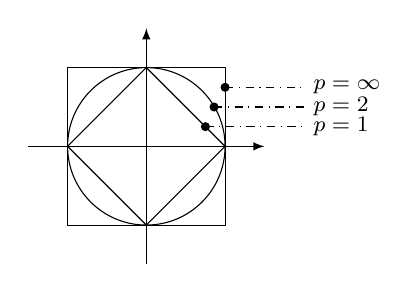
\begin{tikzpicture}
        % axis
        \draw [-latex] (-0.5,1.0) -- (2.5,1.0);
        \draw [-latex] (1.0,-0.5) -- (1.0,2.5);
        % p = inf
        \draw (2.0,0.0) rectangle (0.0,2.0);
        \draw [fill] (2.0,1.75) circle (0.05);
        \draw [dashdotted] (2.0,1.75) -- (3.0,1.75) node [right] {\footnotesize $p=\infty$}; 
        % p = 2
        \draw (1.0,1.0) circle (1.0);
        \draw [fill] (1.86,1.50) circle (0.05);
        \draw [dashdotted] (1.86,1.50) -- (3.0,1.50) node [right] {\footnotesize $p=2$};
        % p = 1
        \draw (1.0,0.0) -- (2.0,1.0) -- (1.0,2.0) -- (0.0,1.0) -- (1.0,0.0);
        \draw [fill] (1.75,1.25) circle (0.05);
        \draw [dashdotted] (1.75,1.25) -- (3.0,1.25) node [right] {\footnotesize $p=1$};
    \end{tikzpicture}
    \caption{Illustration of unit balls with p-norm~$\lVert \mathsf{x} \rVert_{p} = \Big( \sum_{i=1}^{n} |x_{i}|^{p} \Big)^{1/p}$ in an Euclidean space.}
    \label{fig:norm_ball}
\end{figure}

\subsection{Tractable representation of the robust counterpart of an uncertain conic quadratic inequality}

An uncertain conic optimization problem is a collection 
\begin{IEEEeqnarray}{ l }
    \Big\{ \min_{x} \{ c^{T} + d : A_{i} - b_{i} \in \bold{Q}_{i}, \forall i \in 1,...,m \} \Big\}_{(c,d,\{A_{i},b_{i}\}_{i=1}^{m}) \in \UncertaintySet}
\end{IEEEeqnarray}